\documentclass[12pt, titlepage]{article}


\usepackage{amsmath, mathtools}
\usepackage{booktabs}
\usepackage{tabularx}
\usepackage{hyperref}
\hypersetup{
    colorlinks,
    citecolor=black,
    filecolor=black,
    linkcolor=red,
    urlcolor=blue
}
%\usepackage[round]{natbib}
\usepackage[square,sort,comma,numbers]{natbib} 
%% Comments

\usepackage{color}

\newif\ifcomments\commentstrue

\ifcomments
\newcommand{\authornote}[3]{\textcolor{#1}{[#3 ---#2]}}
\newcommand{\todo}[1]{\textcolor{red}{[TODO: #1]}}
\else
\newcommand{\authornote}[3]{}
\newcommand{\todo}[1]{}
\fi

\newcommand{\wss}[1]{\authornote{blue}{SS}{#1}} 
\newcommand{\plt}[1]{\authornote{magenta}{TPLT}{#1}} %For explanation of the template
\newcommand{\an}[1]{\authornote{cyan}{Author}{#1}}

%% Common Parts

\newcommand{\progname}{ProgName} % PUT YOUR PROGRAM NAME HERE %Every program
                                % should have a name



\begin{document}

\title{Test Report: Unit Verification and Validation Plan for Sun Catcher} 
\author{Sharon (Yu-Shiuan) Wu}
\date{\today}
	
\maketitle

\pagenumbering{roman}

\section{Revision History}

\begin{tabularx}{\textwidth}{p{3cm}p{2cm}X}
\toprule {\bf Date} & {\bf Version} & {\bf Notes}\\
\midrule
2019/12.21 & 1.0 & First Version\\
Date 2 & 1.1 & Notes\\
\bottomrule
\end{tabularx}

~\newpage

\section{Symbols, Abbreviations and Acronyms}

\renewcommand{\arraystretch}{1.2}
\begin{tabular}{l l} 
  \toprule		
  \textbf{symbol} & \textbf{description}\\
  \midrule 
  T & Test\\
  \bottomrule
\end{tabular}\\

\wss{symbols, abbreviations or acronyms -- you can reference the SRS tables if needed}

\newpage

\tableofcontents

\listoftables %if appropriate

\listoffigures %if appropriate

\newpage

\pagenumbering{arabic}

This document is the unit testing report for the \progname

\section{Functional Requirements Evaluation}
\begin{enumerate}

\item{InputBounds-id1\\} 
This test is testing the ability of identify the boundary of $\Phi_P$.\\
This result will be display in the ternimal when run the testing.

\begin{table}[h!]
\centering
\noindent \begin{tabular}{l l l l} 
    \toprule		
    \textbf{id} & \textbf{Input} & \textbf{Output}\\ 
	\midrule
   id1.1 &  90  & valid\\
   id1.2 & -90  & valid\\
   id1.3 &  89.9  & valid\\
   id1.4 & -89.9  & valid\\
   id1.5 & 0  & valid\\
   id1.6 & 91  & invalid\\
   id1.7 & -91  & invalid\\
   id1.8 & 90.1  & invalid\\
   id1.9 & -90.1  & invalid\\
    \bottomrule
  \end{tabular}
\caption{Actual Input and Expected Output}
\end{table}


\begin{figure}[hbt!]
 \centering
 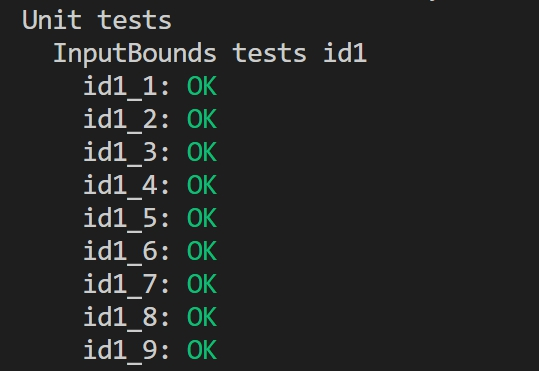
\includegraphics[scale=.5]{InputBounds-id1}
\end{figure}

The result of the test shows that every test cases under Input Bounds-id1 has matched to its expected output. Therefore, the test case success.

\item{InputBounds-id2\\} 
This test is testing the ability of identify the input cases dayT, ($\mathit{year}_\text{Start}$, $\mathit{month}_\text{Start}$, $\mathit{day}_\text{Start}$), whether or not exit in the calender.\\
This result will be display in the ternimal when run the testing.


\begin{table}[h!]
\centering
\noindent \begin{tabular}{l l l l} 
    \toprule		
    \textbf{id} & \textbf{Input} & \textbf{Output}\\ 
	\midrule
   id2.1 & (0, 0, 0) & not exist\\
   id2.2 & (-1, -1, -1)  & not exist\\
   id2.3 & (2020, -1, 29)  & not exist\\
   id2.4 & (2020, 02, -1)  & not exist\\
   id2.5 & (-1, 02, 29)  & not exist\\
   id2.6 & (2020, 13, -1)  & not exist\\
   id2.7 & (2020, 02, 29)  & not exist\\
   id2.8 & (2020, 02, 28)  & exist\\
    \bottomrule
  \end{tabular}
\caption{Actual Input and Expected Output}
\end{table}


\begin{figure}[hbt!]
 \centering
 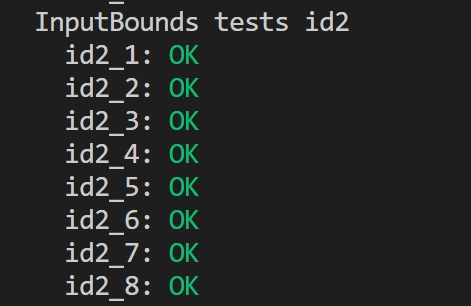
\includegraphics[scale=.5]{InputBounds-id2}
\end{figure}

The result of the test shows that every test cases under Input Bounds-id2 has matched to its expected output. Therefore, the test case success.

\item{InputBounds-id3\\} 
This test is testing the ability of identify the end day whether or not smaller than the start day.\\
This result will be display in the ternimal when run the testing.



\begin{table}[h!]
\centering
\noindent \begin{tabular}{l l l l} 
    \toprule		
    \textbf{id} & \textbf{Input} & \textbf{Output}\\ 
	\midrule
    id3.1 & (2020, 02, 28) - (2021, 02, 28) & valid\\
   id3.2 & (2020, 02, 28) - (2019, 02, 28)  & invalid\\
   id3.3 & (2020, 02, 28) - (2020, 01, 28)  & invalid\\
   id3.4 & (2020, 02, 28) - (2020, 02, 27)  & invalid\\
   id3.5 & (2020, 02, 28) - (2020, 02, 28)  & invalid\\
    \bottomrule
  \end{tabular}
\caption{Actual Input and Expected Output}
\end{table}



\begin{figure}[hbt!]
 \centering
 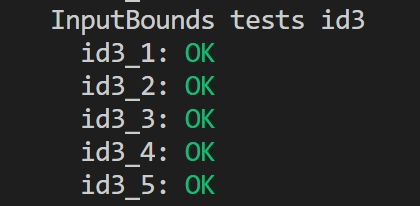
\includegraphics[scale=.5]{InputBounds-id3}
\end{figure}

The result of the test shows that every test cases under Input Bounds-id3 has matched to its expected output. Therefore, the test case success.


\item{calculation-id4\\} 
This is the test case that testing the ability to calculate the Zenith angle.

It is testing by calling the exported access programs, getzenList, under the Calculation Module.\\
The the input can be nd under the path
\../src/tiltAngPro/test/tests"
Input File Name : ``id4.calculation"
Output File Nmae: ``id4.calculation.golden"


\begin{table}[h!]
\centering
\noindent \begin{tabular}{l l l l} 
    \toprule		
    \textbf{id} & \textbf{Input} & \textbf{Output}\\ 
	\midrule
   id4.1 &  43.250943  & 23.250943\\
   id4.2 & -43.250943  & -23.250943\\
   id4.3 & -89.250943  & -69.250943\\
   id4.4 &  89.250943  & 69.250943\\
    \bottomrule
  \end{tabular}
\caption{Actual Input and Expected Output}
\end{table}



\begin{center}
.calculation\\
id4\_1\\
Input 23.250943 Output 23.250943 Absolute Erros = 0.0\\
id4\_2\\
Input -23.250943 Output -23.250943 Absolute Erros = 0.0\\
id4\_3\\
Input -69.250943 Output -69.250943 Absolute Erros = 0.0\\
id4\_4\\
Input 69.250943 Output 69.250943 Absolute Erros = 0.0\\
\end{center}

This result shows that the absolute errors of every test case under calculation-id4 is 0. Therefore, the test case success.

\item{calculation-id5\\}
This is the test case that shows the ability to calculate the sun intensity.

It is testing by calling the exported access programs, sglSunIn, under the Calculation Module.\\
The the input can be nd under the path
\../src/tiltAngPro/test/tests"
Input File Name : ``id5.calculation"
Output File Nmae: ``id5.calculation.golden"


\begin{table}[h!]
\centering
\noindent \begin{tabular}{l l l l} 
    \toprule		
    \textbf{id} & \textbf{Input} & \textbf{Output}\\ 
	\midrule
   id5.1 &  23.250943  & 0.9738212\\
   id5.2 & -23.250943  & 0.9738212\\
   id5.3 & -69.250943  & 0.5786897\\
   id5.4 &  69.250943  & 0.5786897\\
    \bottomrule
  \end{tabular}
\caption{Actual Input and Expected Output}
\end{table}



\begin{center}
.calculation\\
id5\_1\\
Input 0.9738212193883772 Output 0.9738212 \\
Relative Erros = 1.9909586201904972e-8\\
id5\_2\\
Input 0.9738212193883772 Output 0.9738212 \\
Relative Erros = 1.9909586201904972e-8\\
id5\_3\\
Input 0.5786890162786223 Output 0.5786897 \\
Relative Erros = 1.1814991309755385e-6\\
id5\_4\\
Input 0.5786890162786223 Output 0.5786897 \\
Relative Erros = 1.1814991309755385e-6\\
\end{center}

This result shows that the relative error in every case under calculation-id5 is close to 0.
Its satisfies the error tolerance defined in Unit VnV plan. Therefore, the test case success.

\end{enumerate}
\section{Nonfunctional Requirements Evaluation}

\begin{enumerate}
\item code walkthrough : \\
Attendant : Sharon (Yu-Shiuan) Wu, Doctor. Kal\\
Implement Date : 2019/12/19\\
Agenda : \\
\begin{itemize}
\item Check whether or not has the redundant code.
\item Check whether or not the code is readable.
\item Check whether or not the code is implementing with the concise pattern.
\end{itemize}

Conclusion for further improvement:
\begin{itemize}
\item Use lhs2tex to implement the code and the command.
\item Use pattern guard to simplifies the pattern matching.
\item Import external framework, AC-Angle, to convert radian to degree.
\item Use writefile to write the information to the file instead of using appendFile.
\end{itemize}

\end{enumerate}
\subsection{Usability}
		
\subsection{Performance}

\subsection{etc.}
	
\section{Comparison to Existing Implementation}	

This section will not be appropriate for every project.

\section{Unit Testing}

\section{Changes Due to Testing}

\section{Automated Testing}
		
\section{Trace to Requirements}
		
\section{Trace to Modules}		

\section{Code Coverage Metrics}


\bibliographystyle{plain}
\bibliography{../../../refs/References} 

\end{document}